\documentclass{article}
\usepackage[utf8]{inputenc}
\usepackage{listings}
\usepackage{graphicx}

\title{Sistemi Operativi M}
\author{Federico Andrucci}
\date{September 2021}

\begin{document}

\maketitle
\tableofcontents

\section{Virtualizzazione}

Virtualizzare un sistema (hardware e software) significa presentare all'uilizzatore una visione delle risorse del sistema diversa da quella reale.
Ciò è possibile introducendo un \textbf{livello di indirezione} tra la vista logica e quella fisica delle risorse.

Quindi l'obiettivo della virtualizzazione è quello di disaccoppiare il comportamento delle risorsedi un calcolatore dalla loro realizzazione fisica. 
Quindi apparendo diverse da quelle effettive della macchina. Il software che si occupa di virtualizzare in parole semplici divide le risorse reali nel numero di macchine virtuali necessarie. 
Quindi ogni macchina virtuale avrà la sua CPU, GPU, RAM, ecc...

Esmpi di virtualizzazione:
\begin{itemize}
    \item \textbf{Virtualizzazione a livello di processo:} i sistemi multitasking permettono l'esecuzione contemporanea di più processi, ognuno dei quale dispone 
    di una macchina virtuale dedicata. Questo tipo di virtualizzazione viene realizzata dal kernel del sistema operativo.
    \item \textbf{Virtualizzazione della memoria:} in presenza di memoria virtuale, ogni processo vede uno spazio di indirizzamento di dimensioni indipendenti dallo spazio fisico effettivamente a dispozione. Anche questa virtualizzaione è realizzata dal kernel.
    \item \textbf{Astrazione:} un oggetto astratto (risorsa virtuale) è la rappresentazione semplificata di un oggetto (risortsa fisica), quindi esibendo le 
    proprietà significative per l'utilizzatore e nascondendo i dettagli realizzativi non importanti
\end{itemize}

\subsection{Virtualizzazione di un Sistema di Elaborazione}
Tramite la virtualizzazione una singola piattaforma hardware viene condivisa da più elaboratori virtuali, ognuno gestito da un proprio sistema operativo.
Il disaccoppiamento viene realizzato dal \textbf{Virtual Machine Monitor (VMM)}, il cui compito è quello di consentire la condivisione da parte di più macchine 
virtuali di una singola piattaforma hardware.

Quindi il \textbf{VMM} è il \textbf{mediatore unico} nelle interazioni tra le macchine virtuali e
l'hardware, il quale garantisce: \textbf{isolamento tra le VM} e \textbf{stabilità del sistema}.

\subsection{Tecniche del VMM}
\subsubsection{Emulazione}
L'emulazione è l'insieme di tutti quei meccanismi che permettono l'esecuzione di un programma compilato su un determiato sistema di girare su un qualsiasi altro sistema differente da quello nel quale è stato compilato.
Quindi vengono emulate interamente le singole istruzioni dell'architettura ospitata.

I vantaggi dell'emulazione sono l'interoperabilità tra ambienti eterogenei, mentre gli svantaggi sono le ripercussioni sulle performances.

\vspace{5mm}
Esistono principalmente due tecniche di emulazione: \textbf{interpretazione} e \textbf{ricompilazione dimanica}.

\vspace{5mm}
\textbf{Interpretazione}:

L'interpretazione si basa sulla lettura di ogni singola istruzione del codice macchina che deve essere eseguito e sulla esecuzione di più istruzioni sull'host virtualizzante.
Produce un sovraccarico elevento in quanto potrebbero essere necessarie molte istruzioni dell'host per interpretare una singola istruzione sorgente.

\vspace{5mm}
\textbf{Compilazione dinamica}:

Invece di leggere una singola istruzione del sistema ospitato, legge interi blocchi di codice, vengono analizzati, tradotti per la nuova architettura, ottimizzati e messi in esecuzione.
Il vantaggio in termini prestazionali rispetto all'interpretazione è notevolmente maggiore.

Ad esempio parti di codice utilizzati frequentemente vengono bufferizzati nella cache per evitare di doverli ricompilare in seguito.


..
..
..


\subsection{Realizzaione del VMM}
\textbf{Requisiti di Popek e Goldberg del 1974}:

\begin{itemize}
    \item \textbf{Ambiente di esecuzione per i programmi sostanzialmente identico a quello della macchina reale}: Gli stessi programmi che eseguono nel sistema non virtualizzato possono essere eseguiti nelle VM
    senza modifiche e problemi.
    \item \textbf{Garantire un'elevata efficienza nell'esecuzione dei programmi}: Il VMM deve permettere l'esecuzione diretta delle istruzioni impartite dalle macchine virtuali, quindi le istruzioni non 
    privilegiate vengono eseguite direttamente in hardware senza coinvolgere il VMM
    \item \textbf{Garantire la stabilità e la sicurezza dell'intero sistema}: Il VMM deve sempre rimanere sempre nel pieno controllo delle risorse hardware, e i programmi in  esecuzione nelle macchine virtuali non possono 
    accedere all'hardware in modo privilegiato
\end{itemize}

\textbf{Parametri e classificazione}
\begin{itemize}
    \item \textbf{Livello} nel quale è collocato il VMM:
    \begin{itemize}
        \item \textbf{VMM di sistema}: eseguono direttamente sopra l'hardware del elaboratore (vmware, esx, xen, kvm)
        \item \textbf{VMM ospitati}: eseguiti come applicazioni sopra un S.O. esistente (parallels, virtualbox)
    \end{itemize}
    \item \textbf{Modalità di dialogo}: per l'accesso alle risorse fisiche tra le macchine virtuali ed il VMM:
    \begin{itemize}
        \item \textbf{Virtualizzazione pura} (vmware): le macchine virtuali usano la stessa interfaccia dell'architettura fisica
        \item \textbf{Paravirtualizzazione} (xen): il VMM presenta un'interfaccia diversa da quella dell'architettura HW
    \end{itemize}
\end{itemize}

\subsubsection{Ring di protezione}

La CPU prevede due livelli di protezione: \textbf{supervisore o kernel (0)} e \textbf{utente (>0)}.

Ogni ring corrisponde a una diversa modalità di funzionamento del processore:
\begin{itemize}
    \item a livello 0 vengono eseguite le istruzioni privilegiate della CPU
    \item nei ring di livello superiore a 0 le istruzioni privilegiate non vengono eseguite
\end{itemize}

Alcuni progrmmi sono progettati per eseguire nel ring 0, ad esempio il Kernel del S.O. infatti è l'unico componente che ha pieno controllo dell'hardware.

{\large \textbf{VMM (vmm di sistema)}}
In un sistema virtualizzato il VMM deve essere l'unica componente in grado di mantenere il controllo completo dell'hardware. Infatti solo il VMM opera nello stato supervisore, 
mentre il S.O. e le applicazioni eseguono in un ring di livello superiore.

Sorgono però due problemi:
\begin{itemize}
    \item \textbf{Ring deprivileging}: il s.o. della macchina virtuale esegue in un ring che non gli è proprio
    \item \textbf{Ring compression}: se i ring utilizzati sono solo 2, applicazioni e s.o. della macchina virtuale eseguono allo stesso livello: 
    scarsa protezione tra spazio del s.o. e delle applicazioni.
\end{itemize}

\subsubsection{Ring Deprivileging}
Con Ring Deprivilenging si indica una situazione nel quale l'esecuzione di istruzioni privilegiate richieste dal sistema operativo nell'ambiente guest non
possono essere eseguite in quanto richiederebbero un ring 0, ma il kernel della macchina virtuale esegue in un ring di livello superiore (foto telefono 1)

Una possibile prima soluzione è il \textbf{Trap & Emulate}: nel quale se il guest tenta di eseguire un'istruzione privilegiata

\begin{itemize}
    \item la CPU notifica un'eccezione al VMM (\textbf{trap}) e gli trasferisce il controllo
    \item il VMM controlla la correttezza dell'operazione richiesta e ne emula il comportamento (\textbf{emulate})
\end{itemize}

Quindi in poche parole la CPU notifica e delega al VMM il controllo e l'esecuzione dell'istruzione privilegiata.

Esempio:

Il guest tenta di disabilitare le interruzioni (popf), se la richiesta della macchina virtuale fosse eseguita direttamente sulla CPU sarebbero disabilitati
tutti gli interrupt di sistema e quindi il VMM non potrebbe riottenere il controllo. Invece, con Trap&Emulate riceve la notifica di tale richiesta e ne emula
il comportamento sospendendo gli interrupt solamente per la macchina virtuale richiedente.

{\large \textbf{Supporto HW alla virtualizzazione}}
L'archietettura della CPU si dice **naturalmente virtualizzabile** se e solo se prevede l'invio di trap al VMM per ogni istruzione privilegiata invocata da un
livello di protezione differente dal quello del VMM.

Se la CPU è naturalmente virtualizzabile viene implementato il trap&emulate, altrimenti, se non è virtualizzabile vi sono 2 possibilità: **Fast Binary Translation** e 
**Paravirtualizzazione**.

\subsubsection{Fast Binary Translation}
Il VMM scansiona dinamicamente il codice dei sistemi operativi guest prima dell'esecuzione per sostituire a run time i blocchi contenenti istuzioni privilegiate
in blocchi equivalenti dal punto di vista funzionale e contenenti chiamate al VMM. Inoltre i blocchi tradotti sono eseguiti e conservati in cache per eventuali
riusi futuri. (SISTEMARE)

(immagine slide 33)

Il principale limite della Fast Binary Translation è che la traduzione dinamica è molto costosa. Però, con questa tecnica, ogni macchina virtuale è una esatta
copia della macchina fisica, con la possiblità di installare gli stessi s.o. di architetture non virtualizzate.

\subsubsection{Paravirtualizzazione}
Il VMM (hypervison) offre al sistema operativo guest un'interfaccia virtuale (ovviamente differente da quello hardware del processore) chiamata **hypercall API**
alla quale i s.o. guest devono rifersi per avere accesso alle risorse (system call).

Queste Hypercall API permettono di:
\begin{itemize}
    \item richiedere l'esecuzione di istruzioni privilegiate, senza generare un interrupt al VMM
    \item i kernel dei s.o. guest devono quindi essere modificati per avere accesso all'interfaccia del particolare VMM
    \item la struttura del VMM è semplificata perchè non deve più preoccuparsi di tradurre dinamicamente i tentativi di operazioni privilegiate dei s.o. guest
\end{itemize}

Le prestazioni rispetto alla Fast Binary Translation sono notevolmente superiori, però ovviamente c'è una necessità di porting dei dei s.o. guest (non sempre facile).

(aggiungere protezione processore)


\section{La protezione nei Sistemi Operativi}



\section{Programmazione Concorrente}


\section{Modello a memoria comune}

Esistono 2 principali modelli di interazione tra i processi:
\begin{itemize}
    \item Modello a \textbf{memoria comune} (ambiente globale, shared memory)
    \item Modello a \textbf{scambio di messaggi} (ambiente locale, distributed memory)
\end{itemize}

Il modello a memoria comune rappresenta la più semplice astrazione del funzionamento di un sistema in multiprogrammazione costituito da uno o più processi che hanno accesso
ad una memoria comune.

Ogni appliczione viene strutturata come un insieme di componenti, suddiviso in due sottoinsieme disgiunti:
\begin{itemize}
    \item \textbf{Processi} (componenti attivi)
    \item \textbf{Risorse} (componenti passivi)
\end{itemize}

Le Risorse rappresentatno un qualunque oggettim fisico o logico, di cui un processo necessita per portare a termine il suo compito.
Le risorse vengono raggruppate in classi, dove una classe rappresenta l'insieme di tutte e sole le operazioni che un processo può eseguire per operare su risorse di quella classe,

Ovviamente ci deve essere la necessità di specificare quali processi ed in quali istanti possono accedere alla risorsa. Quindi il \textbf{meccanismo di controllo degli accessi}
si occupa di controllare che gli accessi dei processi alle risorse avvengano correttamente.

\subsection{Gestore delle Risorse}

Per ogni risorsa \textbf{R}, il suo gestore definisce, in ogni istante t, \textbf{l'insieme SR(t) dei processi che, in tale istante, hanno il diritto di operare su R}.

\vspace{5mm}

Classificazione delle risorse:
\begin{itemize}
    \item Risorsa R \textbf{dedicata}: se SR(t) ha una caardianlità sempre <= 1
    \item Risorsa R \textbf{condivisa}: in caso contrario
    \item Risorsa R \textbf{allocata staticamente}: se SR(t) è una costante, quindi se SR(t) = SR(t0) per ogni t
    \item Risorsa R \textbf{allocata dinamicamente}: se SR(t) è funzione del tempo
\end{itemize}

\begin{figure}[htbp]
    \centering
    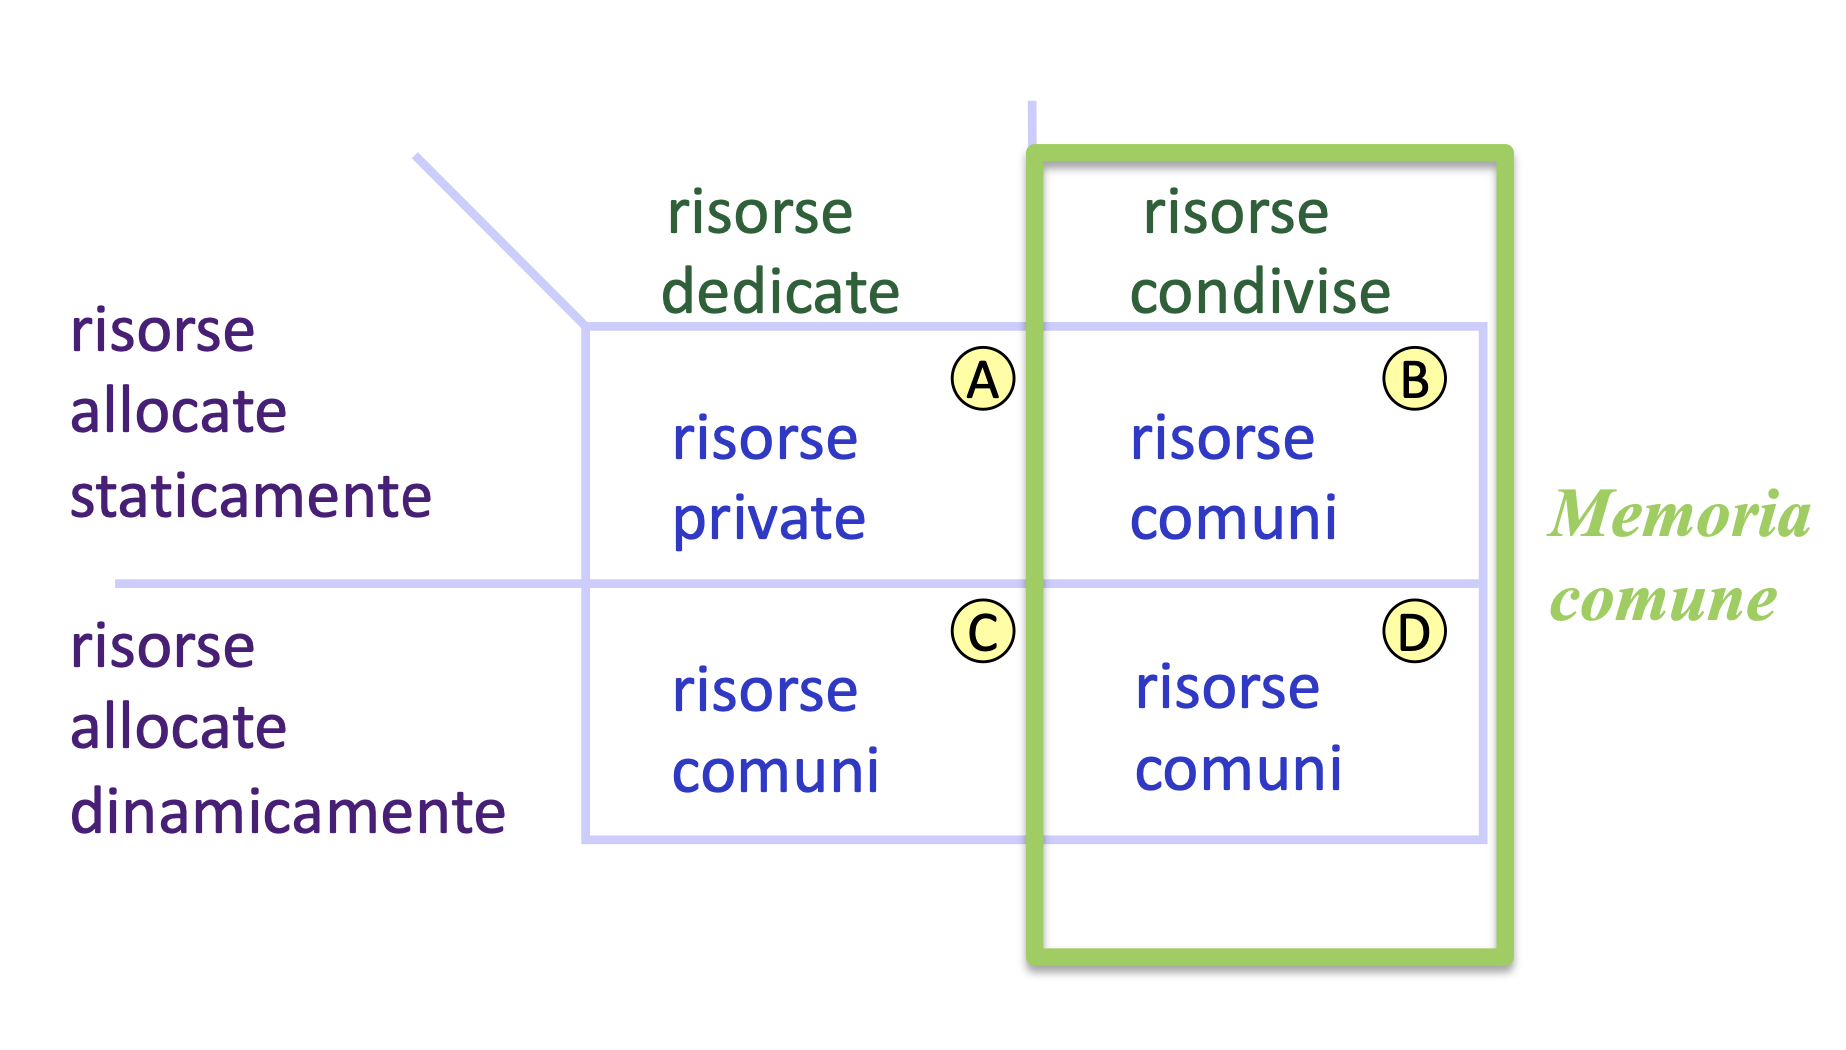
\includegraphics{imgs/tipologie_allocazione.png}
\end{figure}

Per ogni risorsa \textbf{allocata staticamente}, l'insieme SR(t) è definito prima che il programma inizi la propria esecuzione; il gestore della risorsa è il programmatore che,
in base alle regole del linguaggio, stabilisce quale processo può vedere e quindi operare su R.

Per ogni risorsa \textbf{allocata dinamicamente}, il relativo gestore GR definisce l'insieme SR(t) in fase di esecuzione e quindi deve essere un componente della stessa applicazione,
nel quale l'allocazione viene decisa a run-time in base a politiche date.

\vspace{5mm}
Quindi i principali compiti del Gestore delle risorse sono:
\begin{itemize}
    \item mantenere \textbf{aggiornato} l'insieme SR(t) e cioè lo stato di allocazione della risorsa
    \item fornire i \textbf{meccanismi} che un processo può utilizzare per acquisire il diritto di operare sulla risorsa, entrando a far parte dell'insieme SR(t), e per rilasciare
    tale diritto quando non è più necessario
    \item implementare la \textbf{startegia} di allocazione della risorsa e cioè definire quando, a chi e per quanto tempo allocare la risorsa.
\end{itemize}

\vspace{5mm}
{\large \textbf{Accesso a Risorse}}
Consideriamo un processo P che deve operare, ad un certo istante, su una risorsa R di tipo T:

Se R è allocata \textbf{staticamente} a P (modalità A e B), il processo, se appartiene a SR, possiede diritto di operare su R in qualunque istante.
\begin{lstlisting}
R.op(...);
\end{lstlisting}

Se R è allocata \textbf{dinamicamente} a P (modalità C e D), è necessario prevedere un gestore GR, che implementa le funzioni di Richiesta e Rilascio della risorsa; quindi il
processo P deve seguire il seguente protocollo:
\begin{lstlisting}
GR.Richiesta(...);  // acquisizione della risorsa
R.op(...);          // esecuzione dell'operazione op su R
GR.Rilascio(...);   // rilascio della risorsa R
\end{lstlisting}

Se R è allocata come \textbf{risorsa condivisa}, (modalità B e D) è necessario assicurare che gli accessi avvengano in modo non divisibile: nel senso che òe funzioni di accesso alla
risorsa devono essere programmate come una \textbf{classe di sezioni critiche}, utilizzando meccanismi di sincronizzazione offerti dal linguaggio di programmazione e supportati
dalla macchina concorrente.

Se R è allocata come \textbf{risorsa dedicata}, (modalità A e C), essendo P l'unico processo che accede alla risorsa, non è necessario prevedere alcuna forma di sincronizzazione.

\vspace{5mm}
{\large \textbf{Regione critica condizionale [Hoare, Brinch-hansen]}}
Formalismo che permette di esprimere la specifica di qualunque vincolo di sincronizzazione. Data una risorsa R condivisa:

\begin{lstlistin}
region R << Sa; when(C) Sb; >>
\end{lstlisting}

\begin{itemize}
    \item tra doppie parentesi angolai il \textbf{corpo} della region che rappresenta un'operazione da eseguire su una risorsa condivisa R e quindi costituisce una sezione critica
    che deve essere eseguita in \textbf{mutua esclusione} con le altre operazioni definite su R
    \item il corpo della region è costituito da due istruzioni da eseguire in sequenza: l'istruzione \textbf{Sa} e successivamente l'istruzione \textbf{Sb}
    \item in particolare, una volta terminata l'esecizione di Sa viene valutata la condizione \textbf{C}:
    \begin{itemize}
        \item se C è \textbf{vera} l'esecuzione continua con Sb
        \item se C + \textbf{false} il processo che ha invocato l'operazione attende che la condizione C diventi vera. Non appena C sarà vera l'esecuzione della region potrà riprendere
        ed eseguire Sb
    \end{itemize}
\end{itemize}

Esistono però dei casi particolari di regioni critiche:
\begin{itemize}
    \item \textbf{region R << S; >>}: specifica della sola mutua esclusione, senza ulteriori vincoli
    \item \textbf{region R << when(C) >>}: specifica di un semplice vincolo di sincronizzazione, nel quale il processo deve attendere che C sia verificata prima di proseguire
    \item \textbf{region R << when(C) S; >>}: specifica il caso dìin cui la condizione C di sincronizzazione caratterizza lo stato in cui la risorsa R deve trovarsi per poter
    eseguire l'operazione S (C quindi è una precondizione di S)
\end{itemize}

\subsection{Mutua Esclusione}

Il probelma della mutua esclusione nasce quando più di un processo alla volta può e deve accedere a variabili comuni. Quindi è di fondamentale importanza che le operazioni con le quali
i processi accedono alle variabili comuni non si sovrappongano nel tempo.

\end{document}
